\newpage
\setcounter{figure}{0}

\section{Rezultati} % (fold)
\label{sec:Rezultati}

Tijekom izrade diplomskog rada snimljeno je šest scena upotrebom
programa RGBDSlam i iz tih snimaka (slika~\ref{fig:01-all.png}) su
izgrađeni 3D modeli objekata i scena pomoću programa
\texttt{mesh-reconstruction}. Sve snimke i izrađeni modeli nalaze se na
priloženom DVDu. U ovom poglavlju su prikazani rezultati izgradnje i
ispitana je funkcionalnost izgradnje 3D modela scena pomoću 3D kamere.
Za ispitivanje funkcionalnosti metode odabrane su tri scene:
etfos-ured-2013-07-30, etfos-hol-2013-11-20, etfos-hodnik-11-27. Prije
prikaza rezultata potrebno je istaknuti nekoliko problema odnosno
ograničenja ove metode.

Problemi sa načinom stjecanja oblaka točaka
Problemi sa izgradnjom 3D modela 

\begin{figure}[h]
\centering
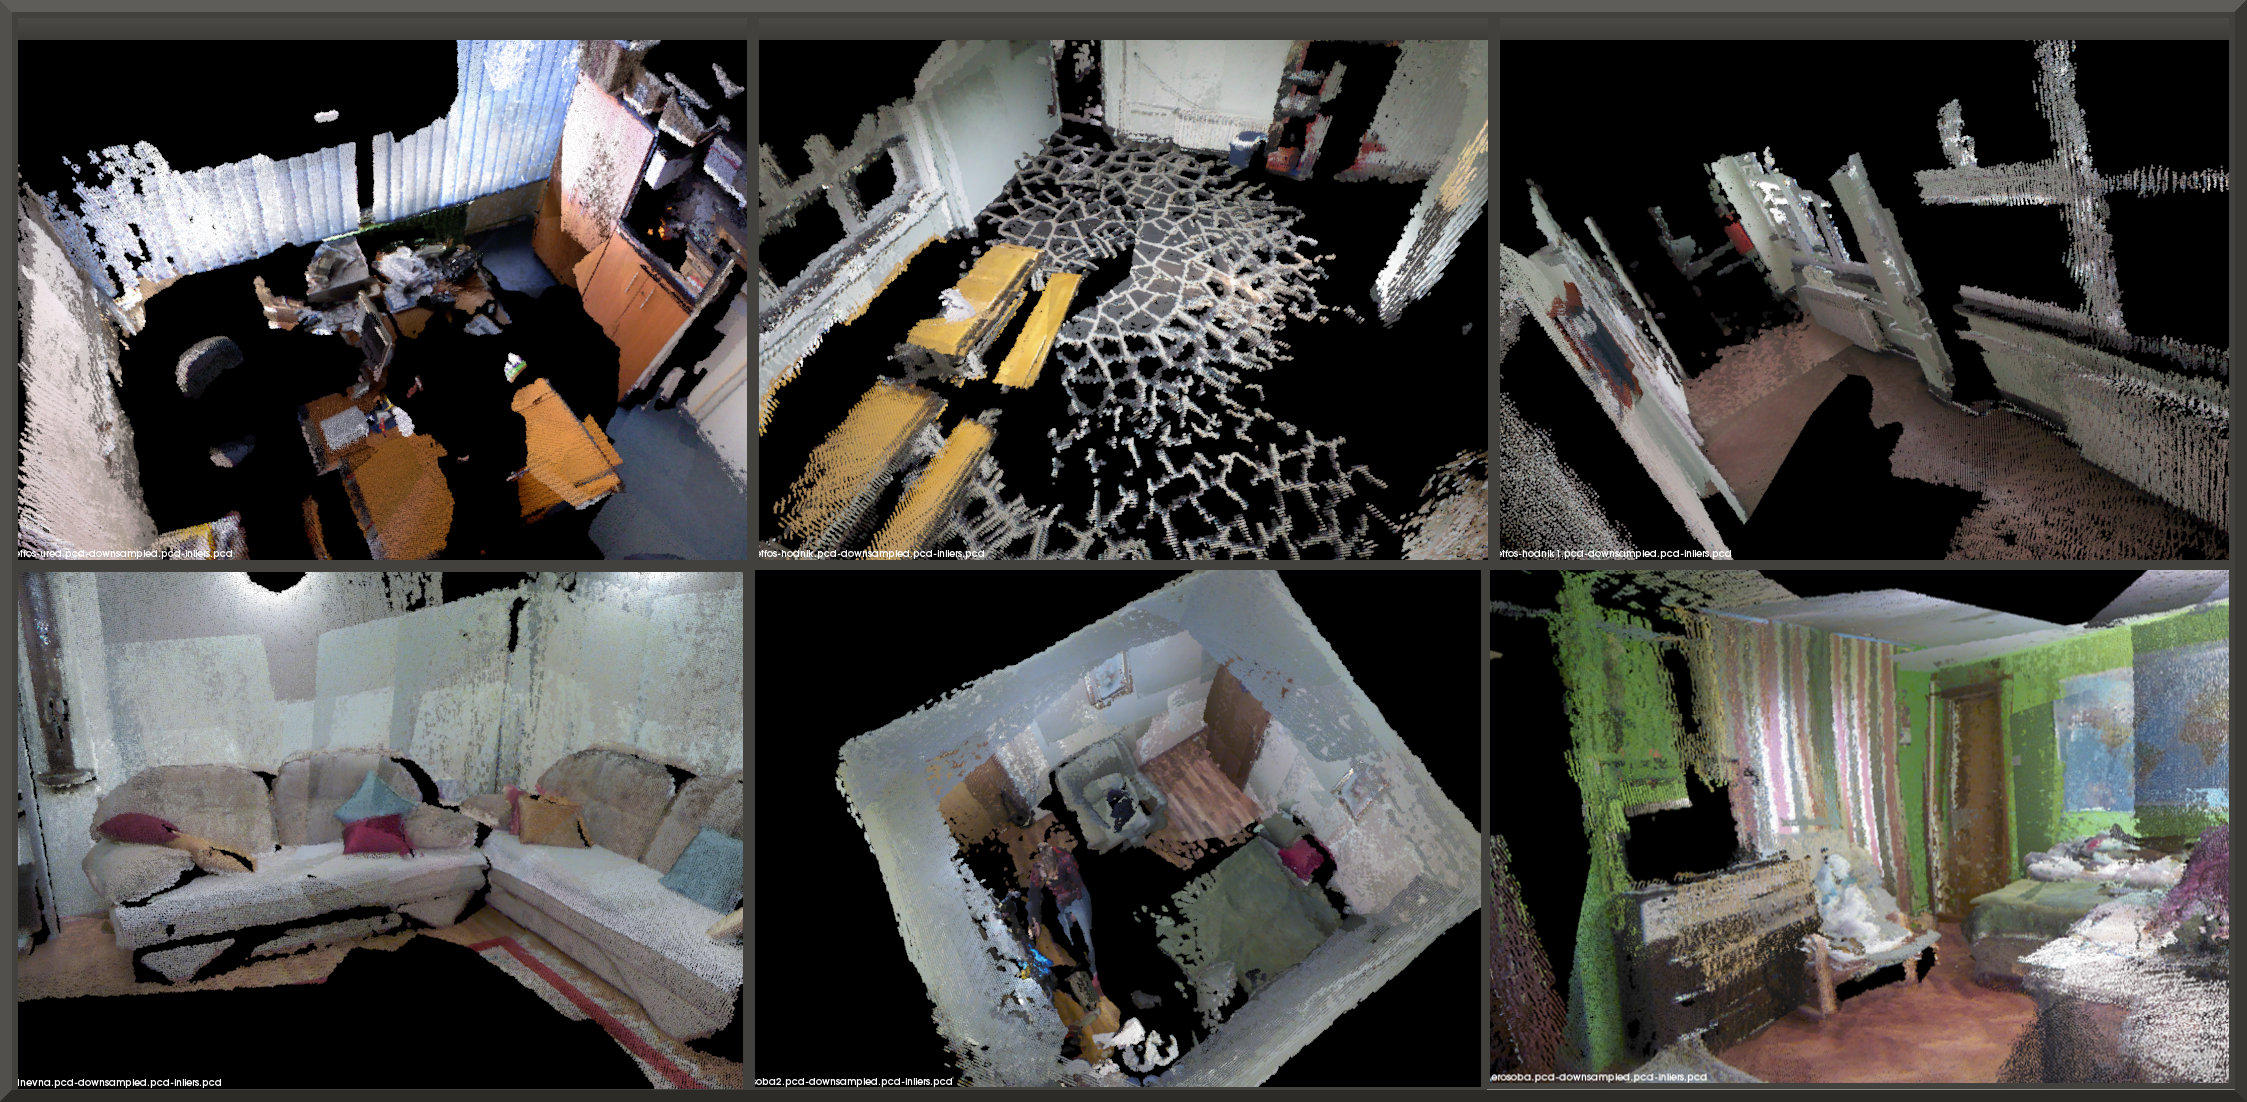
\includegraphics[scale=0.15]{figures/01-all-pcd.png}
\caption{Prikaz svih snimljenih scena}
\label{fig:01-all.png}
\end{figure}

\newpage
\subsection{Prikaz izgrađenih modela scena i objekata} % (fold)
\label{sub:Prikaz izgradenih modela scena i objekata}

\textbf{Snimka: Etfos ured 2013-07-30} 

\begin{figure}[h]
\centering
\includegraphics[scale=0.25]{figures/02-etfos-ured-vtk-pcd-all.png}
\caption{Prikaz izrađenog modela i snimljenog oblaka točaka}
\label{fig:02-etfos-ured-vtk-pcd.png}
\end{figure}

% subsection Prikaz izgrađenih modela scena i objekata (end)

% section Rezultati (end)

